\documentclass[conference,letterpaper,twocolumn]{IEEEtran}
%\usepackage[latin1]{inputenc}
%\usepackage[ansinew]{inputenc}
\usepackage[utf8]{inputenc}

\usepackage{graphicx}
\usepackage{psfrag}
\usepackage{stfloats}
%\usepackage[spanish]{babel}
\usepackage{epsfig}
\usepackage{pifont}
\usepackage{amssymb}
\usepackage{fixltx2e}
\usepackage{amsmath}
\usepackage{rotate}
\usepackage{anysize}
%\usepackage{rotating}
%\usepackage{fancybox}
\usepackage{float}
\usepackage{fancybox}
\usepackage{subfig}

\newcommand{\pig}[1]{\mbox{\boldmath ${#1}$}	}

\newtheorem{Theod}{{\bf Definici\'on}}

\setlength{\oddsidemargin}{5mm}
\setlength{\evensidemargin}{5mm}
\setlength{\topmargin}{4mm}
\setlength{\textwidth}{15cm}
\setlength{\columnsep}{5mm}
\setlength{\textheight}{24cm}





\begin{document}

\title{Modified hypersphere method applied to biparameter homotopy: bipolar circuit simulation}

\author{\authorblockN{H\'ector V\'azquez-Leal and Roberto Casta\~neda Sheissa and Rafael Ravago Vernal}
\authorblockA{Universidad Veracruzana\\
Facultad de Instrumentaci\'on Electr\'onica\\
Xalapa, Veracruz, M\'exico\\
Email: hvazquez@uv.mx}
}

\maketitle

\begin{abstract}
En este artículo se muestra como se puede adaptar y aplicar la técnica de las hiperesferas al trazado de homotopías
multiparametricas. Además,  se presentará una técnica basada en círculos (derivada de las hiperesferas), la cual
es más rápida y simple de implementar que la técnica de las hiperesferas.
Por ultimo, se presentará un análisis comparativo entre ambas técnicas aplicándolas a la simulación
de circuitos con transistores bipolares.
\end{abstract}
 

\section{Introduction} 

El aumento en la complejidad de los circuitos, impulsa el avance científico en el área
de las técnicas de simulación de circuitos integrados. Asimismo, las homotopías se han presentado
como una herramienta novedosa y útil en el área de la solución del punto de operación de circuitos \cite{homo_ArtificialP,homo_iscas05}, debido a que
el método Newton-Raphson (NR) (ampliamente utilizado)  presenta problemas de convergencia como oscilación
y divergencia.

\section{Multiparameter Homotopy}

El primer paso para formular una homotopía es establecer la ecuación de equilibrio a resolver,
la cual se formula a partir de las leyes de kirchhoff quedando definida como:

\begin{equation}
{f}({x})={0} \qquad \text{where} \qquad f:\in \mathfrak{R}^n \to  \mathfrak{R}^n 
\label{fx}
\end{equation}
donde $x$ representa a las variables eléctricas del circuito y $n$ es el número de variables eléctricas.


Las homotopías multiparametricas \cite{homo_DWolfMulti,BLHOM2,homo_dobletrazado} se caracterizan por agregar más de un parámetro homotópico
a la ecuación de equilibrio. Cuando los parámetros homotópicos están ajustados a cero, la solución
de $H(\cdot)$ es trivial y cuando los parámetros alcanzan el valor de uno, entonces se ha localizado
el punto de operación. La funci\'on de homotop\'{\i}a  multiparam\'etrica se puede representar como:

\begin{equation}
{H}({f}({x}),\lambda_1,\lambda_2,...,\lambda_k)=0
\end{equation} 
donde los parámetros homotópicos son $\lambda_1,\lambda_2,...\lambda_k\in[0,1]$ y $k$ es el n\'umero de par\'ametros homot\'opicos.


Las homotopías multiparametricas \cite{homo_DWolfMulti} se han propuesto con la finalidad
de evadir fork bifurcations, singularidades, entre otros problemas que se pueden dar con las trayectorias
homotópicas. Asimismo, tanto para las homotopías uniparametricas \cite{homo_ArtificialP} como para las multiparametricas, la técnica de trazado \cite{homo_hk,homo_allgower}
es una herramienta fundamental que puede afectar la convergencia, velocidad y número de soluciones localizadas.
Por lo tanto, se propone aplicar 2 técnicas de trazado a homotopías multiparametricas, las cuales
serán descritas las próximas secciones.

\section{Técnicas de trazado}

Con la finalidad de aplicar las técnicas de trazado descritas en este artículo se utilizará
a manera de ejemplo una homotopía biparametrica basada en el método homotopía de Newton:
{\small
\begin{equation}
{H}({f}({x}),\lambda_1,\lambda_2 ) =
G (f(x),\lambda_2)-(1-\lambda_1 )G (f(x_i),0) 
\label{hexamp1l}
\end{equation}}
Con la existencia de dos parámetros se produce dos deformaciones o transformaciones
simultaneas y relacionadas una en $G$ y otra en $H$. Cuando $[x,\lambda_1,\lambda_2]=[x_i,0,0]$, 
la función homotópica se satisface ($H(\cdot)=0$).
Además, cuando $[\lambda_1,\lambda_2]=[1,1]$, $G(f(x),1)=f(x)$ y $H(\cdot)=G(f(x),1)$ por lo que la solución
encontrada es precisamente el punto de operación buscado ($x_s$). Sin embargo, como $H:\in \mathfrak{R}^{n+2}\to\mathfrak{R}^n$
tiene 2 variables extras, es necesario agregar otras 2 ecuaciones al sistema $H$ para poder resolverlo con técnicas
más convencionales como NR.
\begin{enumerate}
\item {\bf Ecuación $n+1$}. Se agrega una ecuación que defina la trayectoria $\lambda_1-\lambda_2$, la cual 
se denominará función paramétrica $M(\lambda_1,\lambda_2)$. Esta ecuación cruza por 3 puntos $[\lambda_1,\lambda_2]$:
$p_1=[0,0]$, $p_2=[A,B]$ y $p_3=[1,1]$. La ecuación es:
{
\begin{equation}
\begin{array}{c}
M(\lambda_1,\lambda_2)=-\lambda_{{1}}+\\ { \left( \lambda_{{2}}+{\frac {B \left( - 1+A \right) }
{AB+ 1- 2A}} \right) \over  \left( -{\frac { \left( - 1+ 2\,
A- B \right) \lambda_{{2}}}{AB+ 1- 2A}}+ 2\,{\frac {B
 \left( - 1+A \right) }{AB+ 1- 2A}} \right) }
\end{array}
\label{homotopiaPx4}
\end{equation}
}
donde $p_2$ es definido por usuario, tal como se muestra en la figura \ref{curvasl}(a). 
El rango de valores para $A$ y $B$ es $[0,1]$.
\item {\bf Ecuación $n+2$}. Se agrega la ecuación de la hiperesfera \cite{hiper}:
{\small
\begin{equation}
\begin{array}{c}
S(\cdot)=(x_1-c_1)^2+ (x_2-c_2)^2+ \cdots \\ + (\lambda_1-c_{n+1})^2+(\lambda_2-c_{n+2})^2-r^2
\end{array}
\label{hiperesfera}
\end{equation}
}
donde $\pig{c}$ es el centro
de la hiperesfera (el cual ajusta su valor en cada iteración) y $r\ll 1$ es el radio de la hiperesfera 
(tamaño de paso). 
\end{enumerate}

\begin{figure}[hbtp]
\psfrag{l1}{$\lambda_1$}
\psfrag{l2}{$\lambda_2$}
\psfrag{p1}{$p_1=(0,0)$}
\psfrag{p2}{$p_2=(A,B)$}
\psfrag{p3}{$p_3=(1,1)$}
\centering
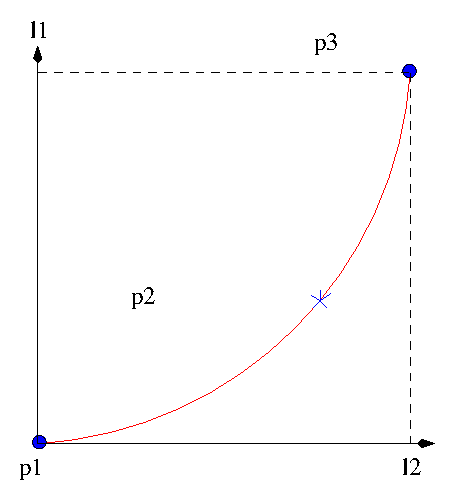
\includegraphics[scale=0.4]{fig/curvasl.eps}
\hspace{5mm}
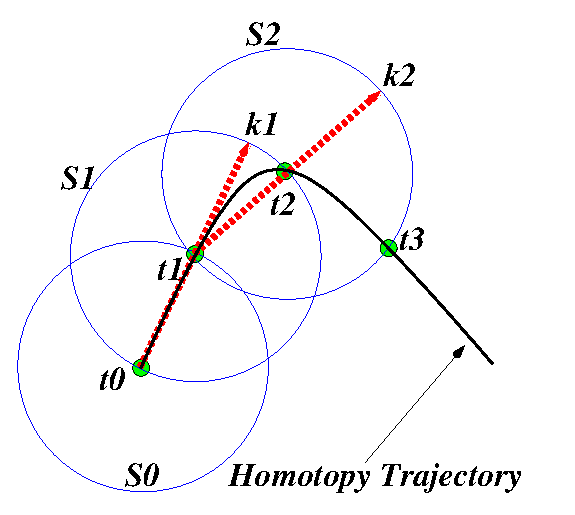
\includegraphics[scale=0.4]{fig/hiper.eps}
\caption{a) Función paramétrica b) Técnica de las hiperesferas}
\label{curvasl}
\end{figure}

El resumen del procedimiento consiste en los siguientes pasos \cite{hiper} (ver figura \ref{curvasl}(b)):

\begin{enumerate}
\item Se  establece la primer hiperesfera $S0$ con centro en $t0=[x_i,p_1]$ y se resuelve el sistema de ecuaciones (ecuaciones \ref{hexamp1l}, \ref{homotopiaPx4} y \ref{hiperesfera})
con el método de NR (usando como punto de inicio el $t0$), localizándose el punto $t1$.
\item Se crea una nueva hiperesfera $S1$ con centro en $t1$.
\item Utilizando los puntos $t0$ y $t1$ se realiza una predicción, la cual toca la hiperesfera $S1$ en el punto $k_1$,
el cual es utilizado como punto de inicio para el método NR, hasta localizar el punto $t_2$ sobre la trayectoria homotópica. 
\item Los pasos 2 y 3 se repiten sucesivamente hasta cruzar por el punto $p_3$.
\item Se utiliza los dos puntos anterior y posterior a $p_3$ para realizar una interpolación \cite{homo_sosonkina}. El tipo de
interpolación utilizada en este artículo es la interpolación lineal multidimensional (conocida como LERP),
la cual produce una aproximación $x_{a}$  de la solución $x_s$ de la ecuación  de equilibrio.
\item Finalmente, usando el método NR con punto de inicio $x_a$, se mejora la precisión del punto de operación $x_s$.
\end{enumerate}

Es posible remplazar la ecuación \ref{hiperesfera} por la ecuación de un circulo, en función de los parámetros homotópicos:

{\small
\begin{equation}
\begin{array}{c}
C(\cdot)=(\lambda_1-c_{n+1})^2+(\lambda_2-c_{n+2})^2-r^2
\end{array}
\label{hiperesfera1}
\end{equation}}
donde $r\ll 1$. El resto de los pasos para implementar la continuación numérica son los mismos que los descritos para la técnica
de las hiperesferas.



\section{Study case: Circuit with bipolar transistors and a diode}

The following circuit \cite{homo_chua} (see figure \ref{newchua}), contains 9 solutions, has become the reference circuit for the Homotopy applied to circuit analysis. 

\begin{figure}[hbtp]
\centering
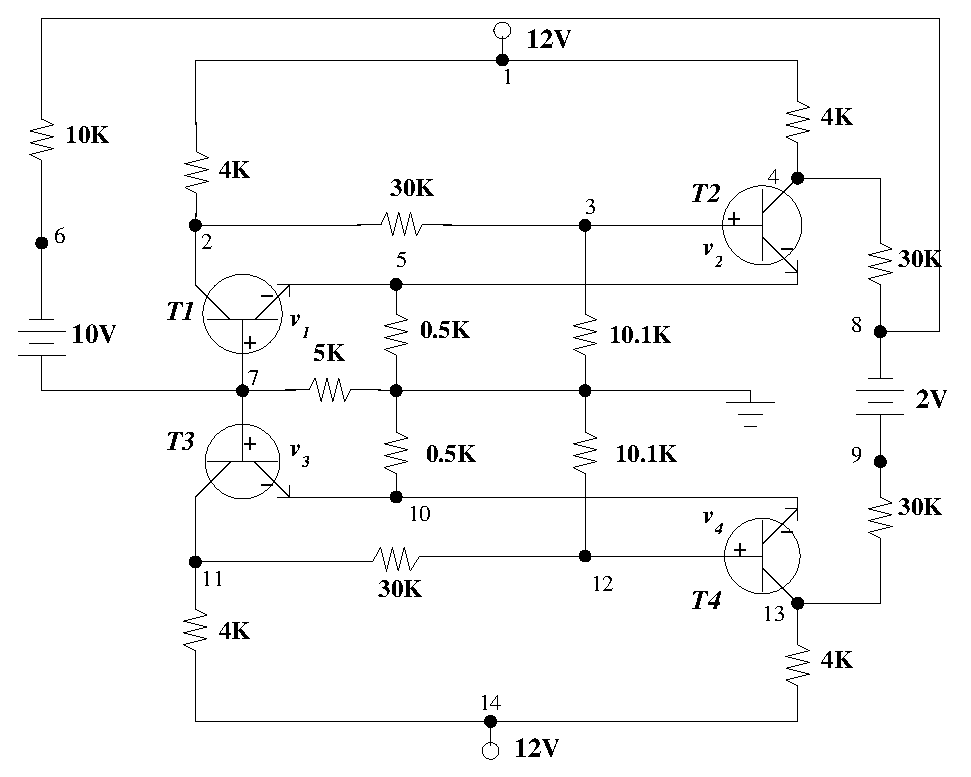
\includegraphics[scale=0.4]{fig/newchua.eps}
\caption{Chua's circuit.}
\label{newchua}
\end{figure}


Utilizando el sistema reportado en \cite{homo_chua} se formula la ecuación de equilibrio aumentada: $\pig{f}(v_1,v_2,v_3,v_4,\lambda_2)$:

{\scriptsize 
\begin{displaymath}
\begin{array}{l}
f_1= 6.103168I_s(e^{40v_1}-1)\lambda_2+4.36634v_2\\
+2.863168I_s(e^{40v_2}-1)-12\\\\
f_2=5.4v_1+3.58I_s(e^{40v_1}-1)\lambda_2+6.62I_s(e^{40v_2}-1)+v_3 \\
+0.7I_s(e^{40v_3}-1)+0.5I_s(e^{40v_4}-1)-22\\\\
f_3=6.103168I_s(e^{40v_3}-1)+2.863168I_s(e^{40v_4}-1)\lambda_2  \\
+4.36634v_4-12\\\\
f_4=v_1+0.7I_s(e^{40v_1}-1)\lambda_2+0.5I_s(e^{40v_2}-1) \\
+5.4v_3+3.58I_s(e^{40v_3}-1)+6.62I_s(e^{40v_4}-1)\lambda_2-20 \\\\
\end{array}
\end{displaymath}
}
donde $I_s=10^{-6}$. Se formula el sistema de ecuaciones aumentado utilizando las ecuaciones \ref{hexamp1l},  \ref{homotopiaPx4} 
y \ref{hiperesfera} o \ref{hiperesfera1} dependiendo de la técnica de trazado a utilizar.

En la tabla \ref{hs1} se presenta de manera resumida los
resultados de realizar el trazado de 4 trayectorias con diferente punto de inicio ($x_{i1}$, $x_{i2}$, $x_{i3}$ y $x_{i4}$) cada una.
Este proceso se repitió para las 2 técnicas de trazado, mostrándose de manera gráfica en las figuras \ref{ht1} (a) y \ref{ht1}(b). Existen dos conclusiones interesantes que resaltar: en primera las trayectorias
homotópicas trazadas desde un mismo punto de inicio conducen exactamente a la misma solución, de hecho,
al contrastar las figuras punto a punto se puede observar que es exactamente la misma trayectoria y
en segunda pese a que las trayectorias son idénticas, la técnica de los círculos requirió de un número fijo de iteraciones 48, lo cuales son mucho menos que los requeridos con la técnica de las hiperesferas. De hecho, de la tabla \ref{hs1} se puede concluir que en el mejor
de los casos (punto de inicio en $x_{i1}$), la técnica de trazado de los círculos resulto tener 10.8 veces menos iteraciones que la técnica de las hiperesferas. En ambas técnicas de trazado se utilizó un radio de $r=0.03$ y una función paramétrica $M$ con $p_2=[0.2,0.3]$.


\begin{table}[tbp]
\center{
{\tiny  \bf
\begin{tabular}{||c|c|c||}
\hline\hline
Hiperesferas Initial P. & \#  & Operating Point $[v_1,v_2,v_3,v_4]$  \\ 
$[\lambda_1,\lambda_2]=[0,0]$ & Iter &  where $[\lambda_1,\lambda_2]=[1,1]$\\ \hline \hline
$x_{i1}$=[-5, -5, -5, -5]  & 519 & $x_{s1}=$[0.3830, -3.5446, 0.3851, -4.0990] \\  \hline
$x_{i2}$=[-1, -2, -1, 0] & 202  & $x_{s2}=$[0.3869, -4.6321, -0.8002, 0.3775] \\  \hline
$x_{i3}$=[-5, -0.5, -5, 0] & 216 & $x_{s3}=$[-0.5136, 0.3775, -0.9682, 0.3775] \\  \hline
$x_{i4}$=[-1, 0, 0, 0] & 168 &$x_{s4}=$[-1.0510, 0.3775, 0.3845, -3.9542]\\  \hline  \hline
Circulos Initial P. & \# & Operating Point  $[v_1,v_2,v_3,v_4]$  \\ 
$[\lambda_1,\lambda_2]=[0,0]$ & Iter & where $[\lambda_1,\lambda_2]=[1,1]$\\ \hline \hline
$x_{i1}$=[-5, -5, -5, -5]  & 48 & $x_{s1}=$[0.3830, -3.5446, 0.3851, -4.0990] \\  \hline
$x_{i2}$=[-1, -2, -1, 0] & 48  & $x_{s2}=$[0.3869, -4.6321, -0.8002, 0.3775] \\  \hline
$x_{i3}$=[-5, -0.5, -5, 0] & 48 & $x_{s4}=$[-0.5136, 0.3775, -0.9682, 0.3775] \\  \hline
$x_{i4}$=[-1, 0, 0, 0] & 48 &$x_{s4}=$[-1.0510, 0.3775, 0.3845, -3.9542]\\  \hline  \hline
\end{tabular}
}
}
\caption{Points Homotopy Simulations}
\label{hs1}
\end{table}

\begin{figure}[hbtp]
\centering
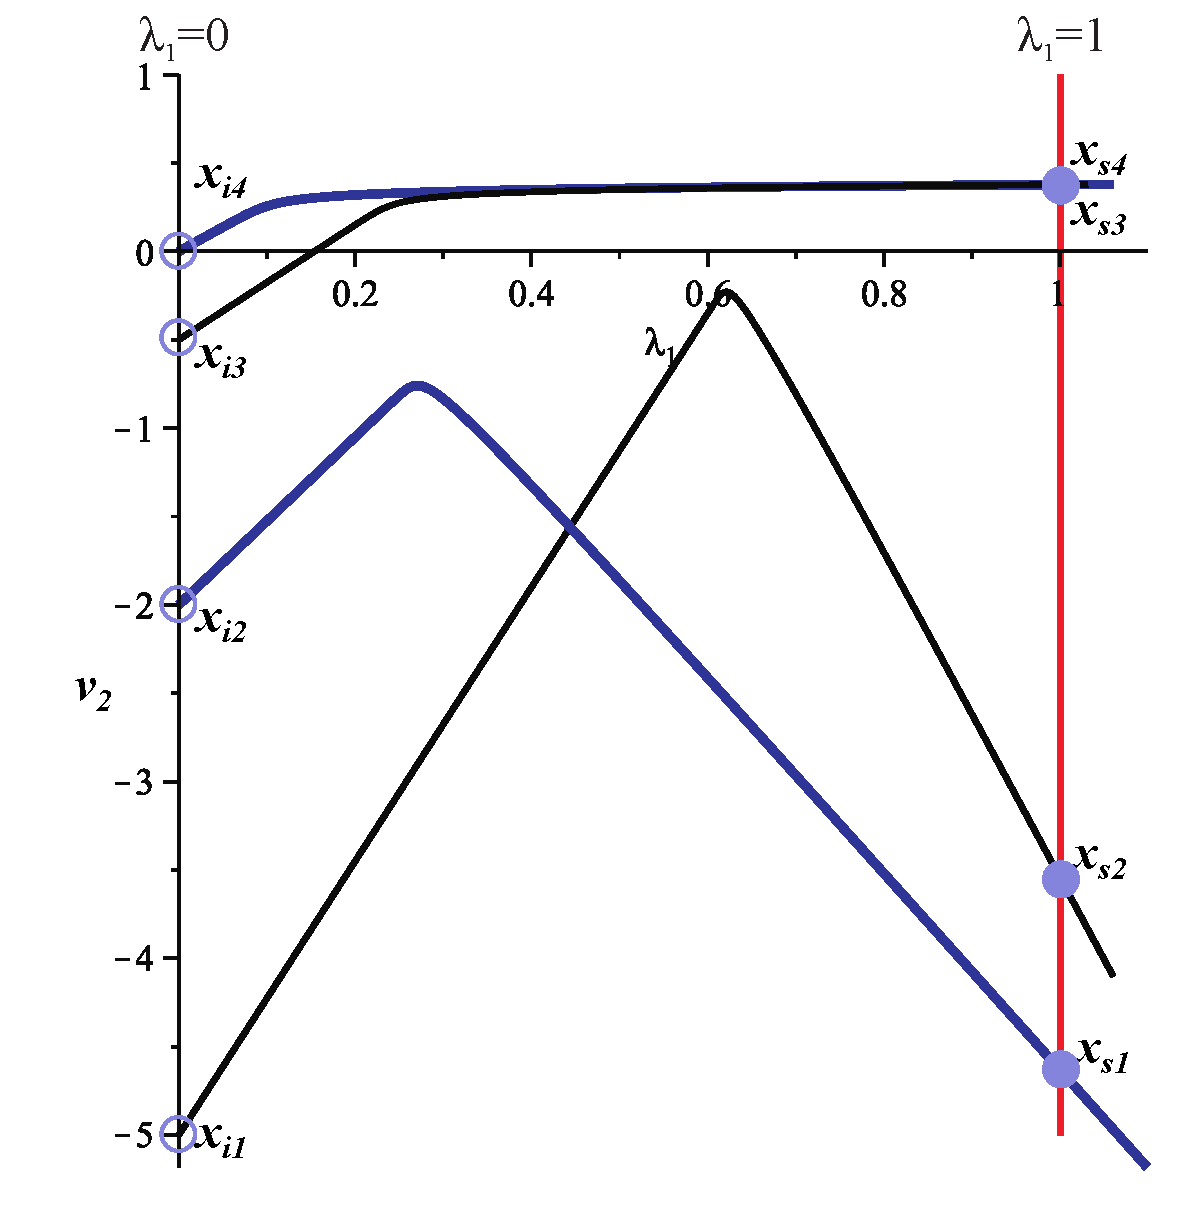
\includegraphics[scale=0.17]{fig/curvasesfera.eps}
%\hspace{5mm}
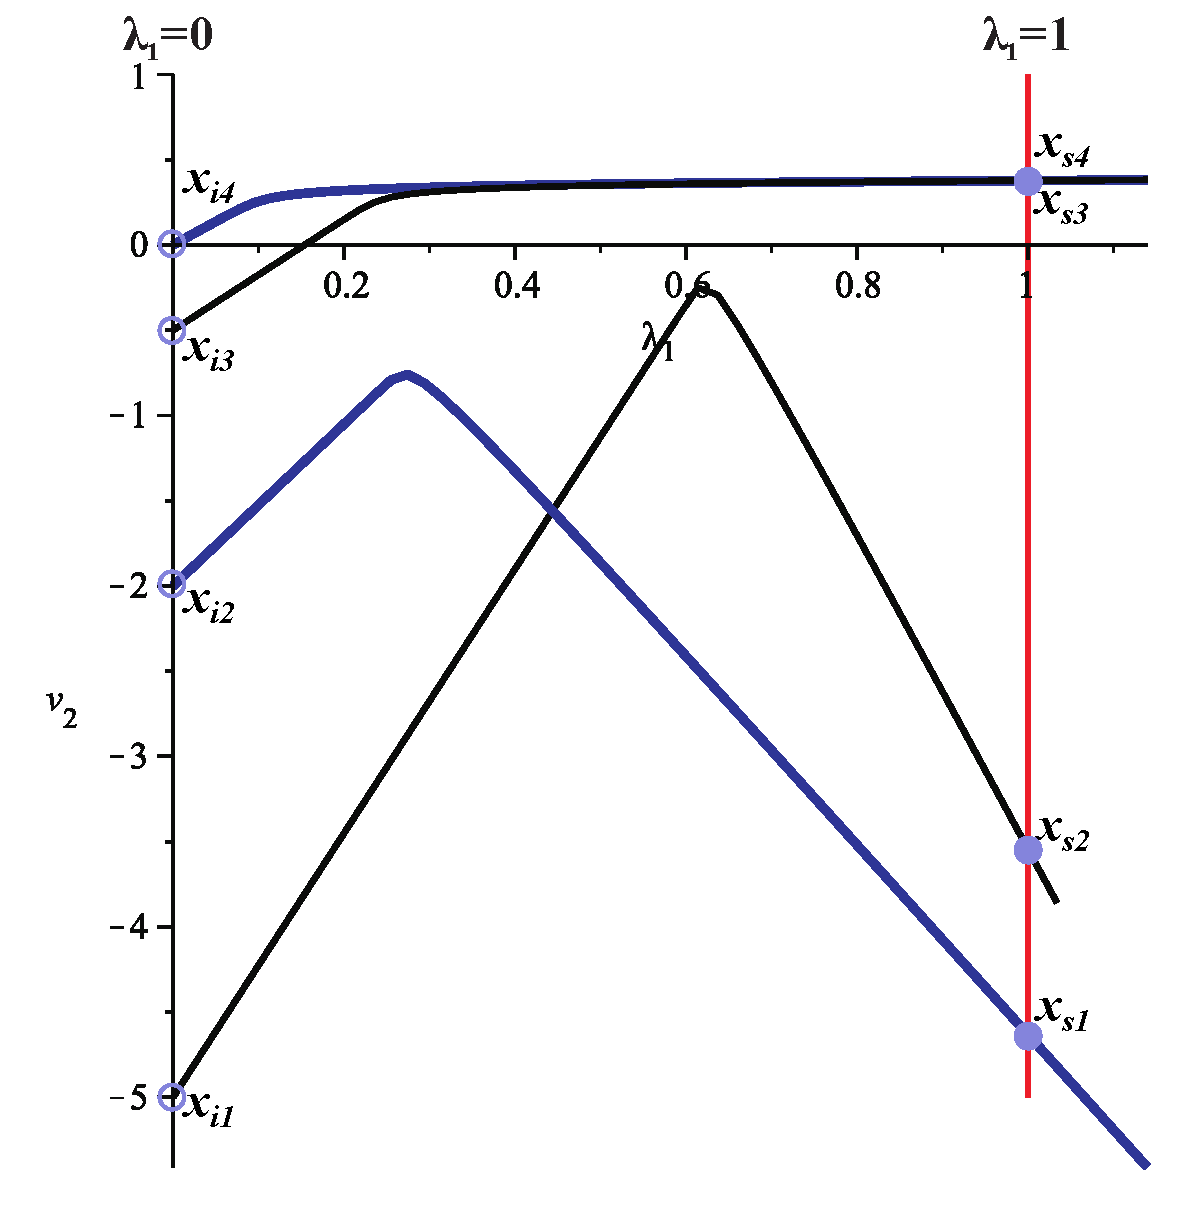
\includegraphics[scale=0.17]{fig/curvascirculo.eps} \\
(a)              \hspace{2cm}          (b)
\caption{Homotopy Trajectories $v_2-\lambda_1$.}
\label{ht1}
\end{figure}

La técnica de los círculos puede ser modifica cambiando uno de los dos parámetros homotópicos
por alguna variable eléctrica de interés. Por ejemplo, se repitió la simulación a partir del punto de inicio $x_{i1}$, cambiando únicamente el circulo de la  ecuación \ref{hiperesfera1}, por otro en función de las variables $v_1$ y $\lambda_1$. El resultado fue que se trazó la trayectoria homotópica ya conocida (ver figura \ref{ht1}(b)) en un total de 191 iteraciones (localizándose la misma solución $x_{s1}$). También es posible utilizar uno de los dos parámetros homotópicos con más de una  variables eléctrica, para
implementar una hiperesfera reducida. Por lo tanto, en un próximo trabajo se abordará con más profundidad este aspecto
de la técnica de los círculos y su posible aplicación a la simulación de circuitos VLSI.




\section{Conclusion}
En el presente trabajo se mostró que es posible utilizar la técnica de las hiperesferas para el trazado de homotopías multiparametricas y se presentó una técnica de trazado derivada derivada de las hiperesferas (circulos), la cual es aún más simple de programar y rápida que la técnica de las hiperesferas. Estos
resultados hacen de la técnica de los círculos una herramienta atractiva para el trazado de funciones multiparametricas.


\bibliographystyle{amsplain}
\bibliography{nh5}

\end{document}
